\section{Anhang}

\subsection{Bodediagramm eines Integrators}

Ein Integrator mit $G(s) = \frac{K}{s}$ hat seine Polstelle bei der Frequenz $\omega = 0$

% TODO Bodeplot auf Integrator anpassen
% \begin{center}
    % Gain
    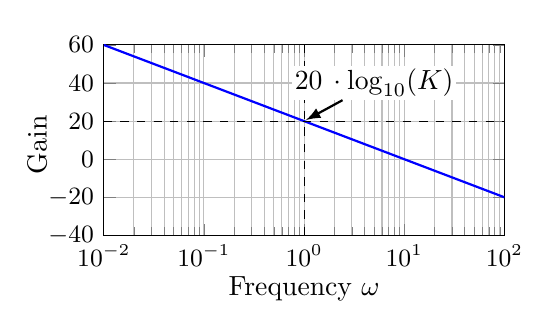
\begin{tikzpicture}
        [%
            scale = 1,
            >=latex
        ]
        \begin{axis}
            [%
                width=.55\columnwidth,
                height=4cm,
                % tick label style
                tick label style={font=\small},
                % x-axis
                xmode=log,
                xmin=0.01, xmax=100, ymin=-40, ymax=60,
                x label style={anchor=north, inner sep=0pt},
                xlabel=Frequency $\omega$,
                xmajorgrids=true,
                xminorgrids=true,
                % y-axis
                y label style={yshift=-1mm, anchor=south, inner sep=0pt},
                ylabel=Gain $\deci \bel$,
                ymajorgrids=true,
                yminorgrids=false
            ]

            % Plot
            \addplot[thick, color=blue, domain=0.01:100]{-20*log10(x)+20};
            
            % guide lines
            \addplot[dashed, color=black, domain=0.01:100]{20}; 
            \addplot [dashed, color=black] coordinates {(1, -40) (1, 60)};
           
            % Node / Label
            \node[inner sep=0pt] (p) at (1, 20) {};
            \node[fill=white, inner sep=1pt] (q) at (5, 40) {$20 \, \deci \bel \cdot \log_{10}(K)$};

            \draw[->, thick, color=black] (q) -- (p);
        \end{axis}
    \end{tikzpicture}
    % Phase
    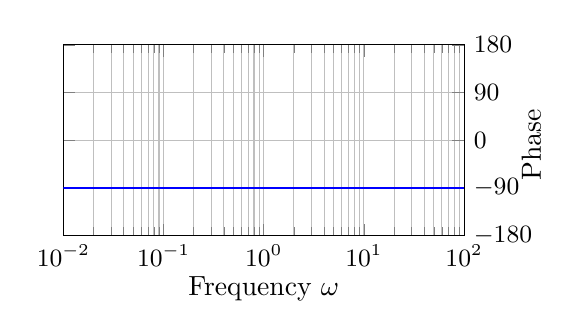
\begin{tikzpicture}
        [%
            scale = 1,
            >=latex
        ]
        \begin{axis}
            [%
                width=.55\columnwidth,
                height=4cm,
                % tick label style
                tick label style={font=\small},
                % x-axis
                xmode=log,
                xmin=0.01, xmax=100, ymin=-180, ymax=180,
                x label style={anchor=north, inner sep=0pt},
                xlabel=Frequency $\omega$,
                xmajorgrids=true,
                xminorgrids=true,
                % y-axis
                y label style={anchor=south, inner sep=0pt},
                ylabel=Phase $\degree$,
                yticklabel pos=right,
                ytick={-180, -90, 0, 90, 180},
                ymajorgrids=true,
                yminorgrids=false
            ]
            
            % Phase
            \addplot[thick, color=blue, domain=0.01:100]{-90};
        \end{axis}
    \end{tikzpicture}
\end{center}

 